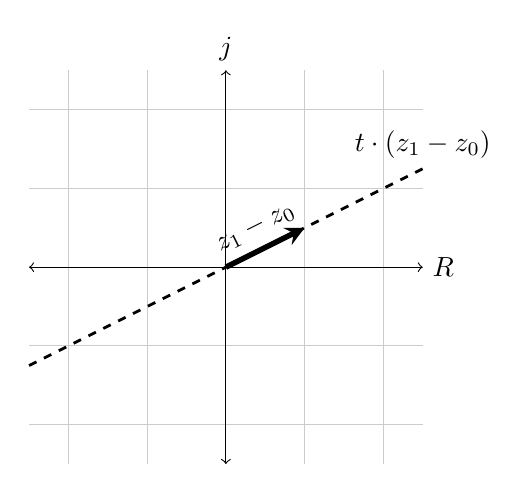
\begin{tikzpicture}
    \draw [thin,gray!40] (-2.5,-2.5) grid (2.5,2.5);
    \draw[<->] (-2.5,0)--(2.5,0) node[right] {$R$};
    \draw[<->] (0,-2.5)--(0,2.5) node[above]{$j$};
    \coordinate (a) at (1,1);
    \coordinate (b) at (3,2);
    \draw[line width=2pt,black,-stealth] (0,0)--(1,0.5) node[midway, above, sloped]{$z_1-z_0$};
    \draw[line width=1pt,black,dashed] (-2.5,-1.25)--(2.5,1.25) node[above]{$t\cdot(z_1-z_0)$};
\end{tikzpicture}
\caption*{Ecuación de la recta sin desplazar}